% Preambulo compartido para clases en formato beamer
\documentclass[9pt, xcolor=svgnames]{beamer}
\usepackage[utf8]{inputenc}
\usepackage[T1]{fontenc}
\usepackage[spanish,es-nodecimaldot]{babel}

\usetheme[progressbar=frametitle]{metropolis}
\metroset{sectionpage=none, subsectionpage=none}
\usepackage{appendixnumberbeamer}
\usepackage{booktabs}
\usepackage{amsmath,amssymb,bm,mathtools}
\usepackage{physics}
\usepackage{graphicx}
\usepackage{multicol}
\usepackage{tikz}
\usepackage{minted}
\usemintedstyle{tango}
\setminted{fontsize=\scriptsize, breaklines=true, linenos=true, bgcolor=LightGray!20, frame=lines}
\newminted{python}{fontsize=\scriptsize, breaklines=true, linenos=true, bgcolor=LightGray!20, frame=lines}
\usepackage{pgfplots}
\pgfplotsset{compat=1.18}
\usepackage{ragged2e}
\usepackage{xspace}
\newcommand{\themename}{\textbf{\textsc{metropolis}}\xspace}

\setbeamercolor{block title}{bg=MidnightBlue!85, fg=white}
\setbeamercolor{block body}{bg=MidnightBlue!5, fg=black}
\setbeamercolor{alerted text}{fg=Crimson}
\setbeamercolor{frametitle}{bg=MidnightBlue!10, fg=black}
\setbeamertemplate{blocks}[rounded][shadow=true]


\weektitle{09}{aprendizaje profundo para datos cientificos}
\titlegraphic{}
\title[PCFI261 -- Semana 09]{\Large Modelos Computacionales PCFI261\\Semana 09: aprendizaje profundo\\para datos cientificos}
\newcommand{\compactcode}{\fontsize{5}{4.7}\selectfont}

\begin{document}

\begin{frame}[plain]
\centering
\vfill
{\Large\bfseries Modelos Computacionales PCFI261}\\[0.25cm]
{\large Semana 09: aprendizaje profundo\\para datos cientificos}\\[0.7cm]
{\large Joaquín Peralta}\\[0.15cm]
{\small \texttt{joaquin.peralta@unab.cl}}\\[0.35cm]
{\small Universidad Andrés Bello}
\vfill
\end{frame}

\begin{frame}{Organizacion de la semana}
\begin{block}{Formato unificado}
La Semana 09 se divide en \textbf{Clase 1} y \textbf{Clase 2}, manteniendo la estructura habitual del curso:
\begin{itemize}
    \item \textbf{30--45 min} de teoria y discusion conceptual.
    \item \textbf{75--90 min} de laboratorio guiado con Python.
\end{itemize}
\end{block}

\vspace{0.2cm}
\begin{columns}[T,onlytextwidth]
\column{0.48\textwidth}
\textbf{Clase 1}
\begin{itemize}
    \item que problema resuelve el deep learning;
    \item representacion de datos, capas y activaciones;
    \item entrenamiento, funcion de perdida y optimizacion;
    \item sobreajuste, particion de datos y escalamiento.
\end{itemize}

\column{0.48\textwidth}
\textbf{Clase 2}
\begin{itemize}
    \item flujo completo con \texttt{tensorflow.keras};
    \item ejemplo autocontenido con un catalogo sintetico;
    \item diagnostico del entrenamiento y decisiones de modelado;
    \item actividades para extender el modelo a problemas del curso.
\end{itemize}
\end{columns}
\end{frame}

\section{Clase 1}

\begin{frame}[plain]
\centering
\vfill
{\Huge \bfseries Clase 1}\\[0.4cm]
{\Large Fundamentos de aprendizaje profundo para fisica y astronomia}
\vfill
\end{frame}

\begin{frame}{Objetivos de la Clase 1}
\begin{itemize}
    \item Distinguir entre \textbf{machine learning clasico} y \textbf{deep learning} en el contexto de datos cientificos.
    \item Interpretar una red neuronal densa como una composicion de transformaciones lineales y no lineales.
    \item Entender el rol de \textbf{features}, \textbf{normalizacion}, \textbf{funcion de perdida} y \textbf{optimizador}.
    \item Identificar sintomas de subajuste y sobreajuste antes de entrenar modelos mas grandes.
\end{itemize}
\end{frame}

\begin{frame}{Por que aparece deep learning en PCFI261}
\begin{columns}[T,onlytextwidth]
\column{0.58\textwidth}
\justifying
En muchos problemas cientificos modernos los datos suelen ser:
\begin{itemize}
    \item series de tiempo;
    \item espectros con muchos canales;
    \item imagenes, mapas o cubos;
    \item simulaciones de alta dimension.
\end{itemize}

\begin{block}{Lectura pedagogica}
El salto no es ``usar una red'', sino permitir que el modelo aprenda parte de la representacion desde los datos.
\end{block}

\column{0.38\textwidth}
\begin{center}
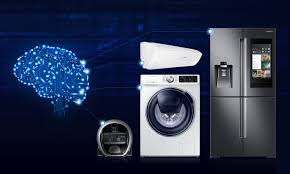
\includegraphics[width=0.88\linewidth]{Figuras/washing.jpeg}
\end{center}

\begin{alertblock}{Idea clave}
Deep learning reduce la dependencia de features diseñadas a mano.
\end{alertblock}
\end{columns}
\end{frame}

\begin{frame}{ML clasico versus deep learning}
\small
\begin{columns}[T,onlytextwidth]
\column{0.48\textwidth}
\begin{block}{Machine learning clasico}
\begin{itemize}
    \item La persona define las \textbf{features}: amplitud, pendiente, color, S/N, etc.
    \item El modelo aprende una regla usando esas variables.
    \item Suele funcionar bien con tablas pequeñas o medianas.
\end{itemize}
\end{block}

\column{0.48\textwidth}
\begin{block}{Deep learning}
\begin{itemize}
    \item La red aprende \textbf{representaciones internas} en varias capas.
    \item Las primeras capas detectan patrones simples; las siguientes combinan patrones.
    \item Es mas util con datos ricos: imagenes, espectros o series largas.
\end{itemize}
\end{block}
\end{columns}

\vspace{0.15cm}
\begin{alertblock}{Diferencia central}
En ML clasico diseñamos la representacion antes de entrenar. En DL entrenamos tambien la representacion, no solo el clasificador o regresor final.
\end{alertblock}

\begin{block}{Regla practica}
Si ya tenemos buenas variables fisicas resumidas, ML clasico puede bastar. Si la informacion esta escondida en datos de alta dimension, DL puede aportar mas.
\end{block}
\end{frame}

\begin{frame}{Una capa densa como operacion matematica}
\begin{columns}[T,onlytextwidth]
\column{0.56\textwidth}
\justifying
Una capa densa recibe un vector de entrada $\bm{x}\in\mathbb{R}^{n}$ y produce
\[
\bm{h} = \phi(W\bm{x} + \bm{b}),
\]
donde:
\begin{itemize}
    \item $W$ es una matriz de pesos;
    \item $\bm{b}$ es un vector de sesgos;
    \item $\phi$ es una funcion de activacion, por ejemplo ReLU o sigmoide.
\end{itemize}

\begin{block}{Lectura computacional}
Cada capa toma un arreglo, mezcla sus componentes mediante una transformacion lineal y luego aplica una no linealidad que permite representar relaciones mas complejas.
\end{block}

\column{0.40\textwidth}
\begin{center}
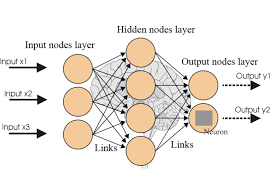
\includegraphics[width=\linewidth]{Figuras/simplenn.png}
\end{center}
\end{columns}
\end{frame}

\begin{frame}{Tensores, shapes y tipos de salida}
\begin{columns}[T,onlytextwidth]
\column{0.54\textwidth}
\begin{itemize}
    \item Un lote de entrenamiento suele verse como una matriz de forma $(N_{\mathrm{batch}}, N_{\mathrm{feat}})$.
    \item En clasificacion binaria la salida suele ser un numero entre 0 y 1.
    \item En regresion la salida puede ser un valor real, por ejemplo una temperatura efectiva o una masa estimada.
    \item El \textbf{shape} correcto es tan importante como la idea fisica del problema.
\end{itemize}

\column{0.42\textwidth}
\begin{tikzpicture}[scale=0.78]
\foreach \y in {0,0.5,1.0,1.5} {
  \foreach \x in {0,0.5,1.0,1.5} {
    \draw[fill=MidnightBlue!10] (\x,\y) rectangle +(0.4,0.4);
  }
}
\node at (1.0,2.3) {\small batch $\times$ features};
\draw[->,thick] (2.4,0.85) -- (3.3,0.85);
\foreach \y in {0.25,0.85,1.45} {
  \draw[fill=Crimson!15] (3.6,\y) circle (0.14);
}
\node at (4.3,2.3) {\small salida};
\end{tikzpicture}
\end{columns}
\end{frame}

\begin{frame}{Activaciones y funcion de perdida}
\begin{columns}[T,onlytextwidth]
\column{0.40\textwidth}
\begin{block}{Activaciones frecuentes}
\begin{itemize}
    \item \textbf{ReLU}: rapida y efectiva en capas ocultas.
    \item \textbf{Sigmoide}: util en salida binaria.
    \item \textbf{Softmax}: util en clasificacion multiclase.
\end{itemize}
\end{block}

\column{0.28\textwidth}
\begin{center}
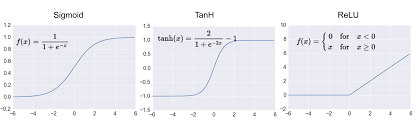
\includegraphics[width=\linewidth]{Figuras/activation.png}
\end{center}

\column{0.28\textwidth}
\begin{block}{Perdidas frecuentes}
\begin{itemize}
    \item \textbf{binary crossentropy} para dos clases;
    \item \textbf{categorical crossentropy} para varias clases;
    \item \textbf{mse} para regresion.
\end{itemize}
\end{block}
\end{columns}

\begin{alertblock}{Criterio practico}
La capa de salida, la activacion y la funcion de perdida deben estar alineadas con la pregunta cientifica.
\end{alertblock}
\end{frame}

\begin{frame}{Entrenamiento, validacion y test}
\justifying
Separar los datos en tres conjuntos evita engañarnos con resultados demasiado optimistas:
\begin{itemize}
    \item \textbf{train}: ajusta los pesos del modelo;
    \item \textbf{validation}: ayuda a elegir hiperparametros y detener el entrenamiento;
    \item \textbf{test}: entrega una estimacion honesta del rendimiento final.
\end{itemize}

\begin{block}{Buena practica}
No mirar el conjunto de test hasta el final. Si lo usamos reiteradamente para decidir, deja de ser una prueba independiente.
\end{block}
\end{frame}

\begin{frame}{Sobreajuste y subajuste}
\begin{columns}[T,onlytextwidth]
\column{0.52\textwidth}
\begin{itemize}
    \item \textbf{Subajuste}: el modelo es demasiado simple o entrena poco.
    \item \textbf{Sobreajuste}: el modelo aprende detalles espurios del conjunto de entrenamiento.
    \item Señales tipicas:
    \begin{itemize}
        \item perdida de entrenamiento baja y validacion alta;
        \item precision de entrenamiento sube mientras validacion se estanca;
        \item sensibilidad extrema al ruido.
    \end{itemize}
\end{itemize}

\column{0.44\textwidth}
\begin{tikzpicture}
\begin{axis}[
    width=5.0cm,
    height=4.2cm,
    xmin=0,xmax=20,
    ymin=0.1,ymax=1.2,
    axis lines=left,
    xtick={0,5,10,15,20},
    ytick={0.2,0.6,1.0},
    xlabel={epoch},
    ylabel={loss},
    tick label style={font=\tiny},
    label style={font=\tiny}
]
\addplot[very thick,MidnightBlue] coordinates {(0,1.05)(4,0.68)(8,0.45)(12,0.31)(16,0.22)(20,0.18)};
\addplot[very thick,Crimson,dashed] coordinates {(0,1.08)(4,0.74)(8,0.53)(12,0.49)(16,0.55)(20,0.66)};
\end{axis}
\end{tikzpicture}
\end{columns}
\end{frame}

\begin{frame}[fragile]{Codigo de apoyo: por que escalar variables}
\inputminted[fontsize=\tiny]{python}{codes/feature_scaling_demo.py}
\end{frame}

\begin{frame}{Cierre Clase 1}
\begin{itemize}
    \item Una red neuronal no es magia: es una composicion de operaciones numericas entrenadas con datos.
    \item En ciencia, el preprocesamiento y la definicion del objetivo siguen siendo tan importantes como la arquitectura.
    \item Antes de usar modelos complejos conviene validar shapes, normalizacion y diagnosticos de generalizacion.
\end{itemize}
\end{frame}

\section{Clase 2}

\begin{frame}[plain]
\centering
\vfill
{\Huge \bfseries Clase 2}\\[0.4cm]
{\Large Taller guiado con \texttt{tensorflow.keras}: de un catalogo sintetico a una clasificacion binaria}
\vfill
\end{frame}

\begin{frame}{Objetivos de la Clase 2}
\begin{itemize}
    \item Implementar un flujo moderno de entrenamiento con \texttt{tensorflow.keras}.
    \item Construir un ejemplo autocontenido inspirado en datos astronomicos tabulados.
    \item Interpretar accuracy, perdida, umbral de clasificacion y matriz de confusion.
    \item Diseñar extensiones realistas hacia datos observacionales o salidas de simulacion.
\end{itemize}
\end{frame}

\begin{frame}{Caso de estudio: catalogo sintetico de transitos}
\justifying
Usaremos un problema sencillo y reproducible: clasificar eventos como
\textbf{transito probable} o \textbf{no transito} a partir de descriptores ya resumidos.

\begin{itemize}
    \item profundidad relativa del evento;
    \item duracion en horas;
    \item razon señal/ruido;
    \item color estelar resumido;
    \item nivel de variabilidad basal.
\end{itemize}

\begin{alertblock}{Advertencia pedagogica}
Este conjunto de datos es sintetico. Sirve para practicar flujo de trabajo y diagnostico, no para afirmar rendimiento cientifico real.
\end{alertblock}
\end{frame}

\begin{frame}{Flujo minimo recomendado}
\begin{enumerate}
    \item generar o cargar datos;
    \item separar en train, validation y test;
    \item escalar variables de entrada;
    \item definir arquitectura y compilar;
    \item entrenar con \texttt{EarlyStopping};
    \item evaluar y revisar errores tipicos.
\end{enumerate}

\begin{block}{Buena practica de curso}
Guardar el preprocesamiento y el umbral de decision junto con el modelo evita que el pipeline quede incompleto.
\end{block}
\end{frame}

\begin{frame}[fragile]{Codigo principal: datos y particion}
\inputminted[firstline=8,lastline=43,fontsize=\compactcode]{python}{codes/stellar_catalog_mlp.py}
\end{frame}

\begin{frame}[fragile]{Codigo principal: arquitectura y entrenamiento}
\inputminted[firstline=45,lastline=77,fontsize=\compactcode]{python}{codes/stellar_catalog_mlp.py}
\end{frame}

\begin{frame}[fragile]{Codigo principal: evaluacion y diagnostico}
\inputminted[firstline=79,lastline=96,fontsize=\tiny]{python}{codes/stellar_catalog_mlp.py}
\end{frame}

\begin{frame}{Que deberiamos mirar en los resultados}
\begin{itemize}
    \item \textbf{loss} y \textbf{val\_loss}: miden estabilidad del entrenamiento.
    \item \textbf{accuracy}: util, pero insuficiente si las clases estan desbalanceadas.
    \item \textbf{confusion matrix}: muestra falsos positivos y falsos negativos.
    \item \textbf{threshold}: cambiar el umbral altera el compromiso entre sensibilidad y precision.
\end{itemize}

\begin{block}{Pregunta cientifica}
En un pipeline de deteccion, \textquestiondown preferimos perder candidatos reales o revisar mas falsos positivos? La respuesta depende del costo experimental y del objetivo fisico.
\end{block}
\end{frame}

\begin{frame}{Conexiones naturales con PCFI261}
\begin{itemize}
    \item Clasificar curvas de luz o eventos transientes a partir de features resumidas.
    \item Regresion de parametros fisicos a partir de espectros o salidas de simulacion.
    \item Autoencoders para reducir dimensionalidad de snapshots de simulaciones.
    \item Redes convolucionales para imagenes astronómicas o mapas 2D.
\end{itemize}

\begin{alertblock}{Criterio de modelacion}
La red es una herramienta. La pregunta fisica, la calidad de las etiquetas y la estrategia de validacion siguen mandando.
\end{alertblock}
\end{frame}

\begin{frame}{Actividades propuestas}
\begin{enumerate}
    \item \textbf{Base}: ejecutar el ejemplo con dos capas ocultas y reportar accuracy, precision y recall.
    \item \textbf{Exploracion}: variar numero de neuronas, tasa de aprendizaje y batch size.
    \item \textbf{Umbral}: comparar resultados con umbrales 0.3, 0.5 y 0.7.
    \item \textbf{Extension}: reformular el problema como regresion para predecir un parametro continuo.
    \item \textbf{Desafio}: reemplazar el catalogo sintetico por un dataset propio del curso y justificar el pipeline.
\end{enumerate}

\begin{block}{Entregable sugerido}
Notebook o script con metricas, figuras, breve discusion de errores y reflexion sobre como cambiaria el experimento con datos reales.
\end{block}
\end{frame}

\begin{frame}{Comentarios docentes}
\begin{itemize}
    \item Conviene enfatizar que \texttt{predict\_classes} ya no se usa: hoy se umbraliza la salida de \texttt{model.predict}.
    \item Si el estudiantado no tiene TensorFlow instalado, el flujo puede discutirse primero leyendo el codigo y luego ejecutarse en un entorno preparado.
    \item La semana queda mejor conectada con PCFI261 si la actividad final se ata a catalogos, curvas de luz o salidas de simulacion ya vistas en el curso.
\end{itemize}
\end{frame}

\begin{frame}{Cierre de la semana}
\begin{itemize}
    \item Modernizar deep learning no significa usar modelos mas grandes, sino usar mejores practicas.
    \item Un pipeline reproducible requiere separar datos, escalar, monitorear validacion y documentar decisiones.
    \item Esta semana deja una base util para pasar luego a imagenes, series de tiempo o problemas de regresion cientifica.
\end{itemize}
\end{frame}

\end{document}
